\documentclass[a4paper]{article}

\usepackage[english]{babel}
\usepackage[utf8]{inputenc}
\usepackage{amsmath}
\usepackage{enumitem}
\usepackage{graphicx}
\usepackage{amsmath,amsfonts,amssymb}
\usepackage[colorinlistoftodos]{todonotes}

\title{ECE 498 - Homework 1: Math Basics}

\author{Amod Agrawal, amodka2}

\date{\today}

\begin{document}
\maketitle

\hfill \newline
\textbf{Problem 1.}\\ 
\newline \hfill
Q1. False \newline
The null space of the matrix depends on the column space. In this case since m \textless n, implies rank r \textless n. This means there will exist linearly dependent columns: hence null space won't be zero.\\ 
\newline \hfill
Q2. False \newline
It subtracts twice of second column from first column.\\ 
\newline \hfill
\begin{align}
 B &=  
\begin{bmatrix}
    b_{11} & b_{12} & b_{13} \\
   b_{21} & b_{22} & b_{23} \\
   b_{31} & b_{32} & b_{33} \\
\end{bmatrix}
\end{align}

\begin{align}
B \cdot A &=  
\begin{bmatrix}
   b_{11} & b_{12} & b_{13} \\
   b_{21} & b_{22} & b_{23} \\
   b_{31} & b_{32} & b_{33} \\\end{bmatrix}
\cdot
\begin{bmatrix}
   1 & 0 & 0 \\
   -2 & 0 & 0 \\
   0 & 0 & 1 \\
\end{bmatrix}
\end{align}

\begin{align}
 =  
\begin{bmatrix}
   b_{11} - 2 b_{12} & b_{12} & b_{13} \\
   b_{21} - 2 b_{22} & b_{22} & b_{23} \\
   b_{31} - 2 b_{32} & b_{32} & b_{33} \\
   \end{bmatrix}
\end{align}

\hfill \newline
Q3. True \newline
\begin{align}
Q \cdot Q\textsuperscript{T} = I (Orthonormal)\\
Q \cdot Q\textsuperscript{-1} = I   (Inverse)
\end{align}

\begin{align}  
\begin{bmatrix}
   - & A & -\\
   - & B & - \\
   - & C & - \\\end{bmatrix}
\cdot
\begin{bmatrix}
   | & | & | \\
   A & B & C \\
   | & | & | \\
\end{bmatrix}
=
\begin{bmatrix}
   1 & 0 & 0 \\
   0 & 1 & 0 \\
   0 & 0 & 1 \\
\end{bmatrix}
\end{align}
\begin{align}
A\textsuperscript{2} = 1, B\textsuperscript{2} = 1, C\textsuperscript{2} = 1 
\end{align}

\hfill \newline
Q4. False\newline
Convolution in time domain = multiplication in frequency domain: \\
S1 has f1, f2, f3 and S2 has f2, f3, f4.\\
$S1 \cdot $S2 will only have f2 and f3. \\ 

\hfill \newline
Q5. True\newline
By definition, the vectors of a basis (b1, b2, b3) are linearly independent and the null space is 0. c1, c2, c3 must be zero. 

\hfill \newline
Q6. False \newline
Dividing a vector by its norm (magnitude) will give us the unit vector. Hence, the length of the resulting vector will be 1 and not 0.

\hfill \newline
\textbf{Problem 2.}\\ \newline
A matrix M is symmetric if M = M\textsuperscript{T}.\newline Let M = A\textsuperscript{T}A.\\
M\textsuperscript{T} = (A\textsuperscript{T}A)\textsuperscript{T} = A\textsuperscript{T}A = M. \hfill \{(AB)\textsuperscript{T} = B\textsuperscript{T}A\textsuperscript{T}\}\\
Hence, A\textsuperscript{T}A is symmetric.

\hfill \newline
\textbf{Problem 3.}\\ \newline

The two equations are:
\begin{equation}
3x + 2y = 10
\end{equation}
\begin{equation}
6x + 4y = b
\end{equation}

In terms of matrices of form $A \cdot $X = B : 
\begin{align}  
\begin{bmatrix}
   3 & 2\\
   6 & 4 \\
 \end{bmatrix}
\cdot
\begin{bmatrix}
  x \\
  y\\ 
 \end{bmatrix}
=
\begin{bmatrix}
 10\\
 b\\
\end{bmatrix}
\end{align}

The columns of the matrix A are linearly dependent: 
\begin{align}
\frac{3}{2}
\cdot
\begin{bmatrix}
  2\\
  4\\ 
 \end{bmatrix}
 = 
 \begin{bmatrix}
  3\\
  6\\ 
 \end{bmatrix}
\end{align}

For the equation to have a solution b must lie in the column space of A which is:
\begin{align}
c
\cdot
\begin{bmatrix}
  1\\
  2\\ 
 \end{bmatrix}
\end{align}

Hence, for b = 20, we have one solution. This is the only value that lies in the column space of A.\\
For any value of b other than b = 20, we won't have a solution because it won't lie in column space of A.\\


\hfill \newline
\textbf{Problem 4.}\\
The given equations are:
\begin{equation}
 x - y = 2
\end{equation}
\begin{equation}
 x + y = 4
\end{equation}
\begin{equation}
 2x + y = 8
\end{equation}

In matrix form of $A \cdot $X = b:
\begin{align}  
\begin{bmatrix}
   1 & -1\\
   1 & 1 \\
   2 & 1\\
 \end{bmatrix}
\cdot
\begin{bmatrix}
  x\\
  y\\ 
  z\\
 \end{bmatrix}
=
\begin{bmatrix}
2\\
 4\\
8\\
\end{bmatrix}
\end{align}

The solution for the given equations do not exist and hence there we try to use least squares to minimize error. X\textsuperscript{*} gives us the least square solution in the following equation:
\begin{equation}
(A^{T} \cdot A) \cdot X^{*} = A^{T} \cdot B
\end{equation}

\begin{align} 
A\textsuperscript{T}A =
\begin{bmatrix}
   1 & 1 & 2\\
   -1 & 1 & 1 \\
 \end{bmatrix}
 \cdot
 \begin{bmatrix}
   1 & -1\\
   1 & 1 \\
   2 & 1\\
 \end{bmatrix} 
 =
\begin{bmatrix}
   6 & 2\\
   2 & 3 \\
 \end{bmatrix}
\end{align}

\begin{align} 
A\textsuperscript{T}B=
\begin{bmatrix}
   1 & 1 & 2\\
   -1 & 1 & 1 \\
 \end{bmatrix}
 \cdot
 \begin{bmatrix}
   2\\
   4\\
   8\\
 \end{bmatrix} 
 =
\begin{bmatrix}
   22\\
   10\\
 \end{bmatrix}
\end{align}


\begin{align}
\begin{bmatrix}
   6 & 2 & | & 22 \\
   2 & 3 & | & 10\\
 \end{bmatrix}
 \rightarrow
 \begin{bmatrix}
   1 & 0 & | & \frac{23}{7} \\
   0 & 1 & | & \frac{8}{7}\\
 \end{bmatrix}
\end{align}

Least square solutions:
\begin{equation}
x = \frac{23}{7} ; y=\frac{8}{7}
\end{equation}

\hfill \newline
\textbf{Problem 5.}\\
In the Fourier Matrix F:
\begin{equation}
F\textsubscript{mn} = e^{-j \cdot \frac{2 \pi}{N} \cdot m \cdot n}
\end{equation}

Hence, an F\textsubscript{4x4} for 0$\leq$ m $\leq$3 and 0$\leq$ n $\leq$ 3:
\begin{align}
F\textsubscript{mn} =
\begin{bmatrix}
    e^{-j \cdot \frac{2 \pi}{N} \cdot 0 \cdot 0}& e^{-j \cdot \frac{2 \pi}{N} \cdot 1 \cdot 0} & e^{-j \cdot \frac{2 \pi}{N} \cdot 2 \cdot 0} & e^{-j \cdot \frac{2 \pi}{N} \cdot 3 \cdot 0} \\
   e^{-j \cdot \frac{2 \pi}{N} \cdot 0 \cdot 1} & e^{-j \cdot \frac{2 \pi}{N} \cdot 1 \cdot 1} &e^{-j \cdot \frac{2 \pi}{N} \cdot 2 \cdot 1}  &e^{-j \cdot \frac{2 \pi}{N} \cdot 3 \cdot 1}\\
     e^{-j \cdot \frac{2 \pi}{N} \cdot 0 \cdot 2} & e^{-j \cdot \frac{2 \pi}{N} \cdot 1 \cdot 2} &e^{-j \cdot \frac{2 \pi}{N} \cdot 2 \cdot 2}  &e^{-j \cdot \frac{2 \pi}{N} \cdot 3 \cdot 2}\\
  e^{-j \cdot \frac{2 \pi}{N} \cdot 0 \cdot 3} & e^{-j \cdot \frac{2 \pi}{N} \cdot 1 \cdot 3} &e^{-j \cdot \frac{2 \pi}{N} \cdot 2 \cdot 3}  &e^{-j \cdot \frac{2 \pi}{N} \cdot 3 \cdot 3}\\
\end{bmatrix}
\end{align}

\begin{align}
F\textsubscript{4} =
\begin{bmatrix}
	1 & 1 & 1 & 1\\
	1 & -j & -1 & j\\
	1 & -1 & 1 & -1\\
	1 & j & -1 & -j\\
 \end{bmatrix}
\end{align}

\begin{align}
=
\begin{bmatrix}
	1 & 1 & 1 & 1\\
	1 & -j & -1 & j\\
	1 & -1 & 1 & -1\\
	1 & j & -1 & -j\\
 \end{bmatrix}
 \cdot
 \begin{bmatrix}
	1\\
	2\\
	3\\
	4\\
 \end{bmatrix}
 =
 \begin{bmatrix}
	10\\
	-2 + 2j\\
	-2\\
	-2 - 2j\\
 \end{bmatrix}
\end{align}

\begin{align}
FFT (
 \begin{bmatrix}
	1\\
	2\\
	3\\
	4\\
 \end{bmatrix}
 ) =
 \begin{bmatrix}
	10\\
	-2 + 2j\\
	-2\\
	-2 - 2j\\
 \end{bmatrix}
 \end{align}
 
 
\begin{align}
Inverse(F\textsubscript{4}) = F\textsuperscript{-1} = (F\textsuperscript{*})\textsuperscript{T} = 
\begin{bmatrix}
	1 & 1 & 1 & 1\\
	1 & j & -1 & -j\\
	1 & -1 & 1 & -1\\
	1 & -j & -1 & j\\
 \end{bmatrix}
\end{align}

Time domain signal = 

\begin{align}
\frac{1}{4}
\begin{bmatrix}
1 & 1 & 1 & 1\\
	1 & j & -1 & -j\\
	1 & -1 & 1 & -1\\
	1 & -j & -1 & j\\
 \end{bmatrix}
 \cdot
 \begin{bmatrix}
 0\\
 0\\
 1\\
 0\\
 \end{bmatrix}
 = 
 \frac{1}{4}
 \begin{bmatrix}
 1\\
 -1\\
 1\\
 -1\\
 \end{bmatrix}
\end{align}

\begin{align}
IFFT(
 \begin{bmatrix}
 0\\
 0\\
 1\\
 0\\
 \end{bmatrix}
)
=
 \begin{bmatrix}
 \frac{1}{4}\\\\
  \frac{-1}{4}\\\\
  \frac{1}{4}\\\\
  \frac{-1}{4}\\
 \end{bmatrix}
\end{align}

\hfill \newline
\textbf{Problem 6.}\\

\begin{equation}
Z\textsubscript{m} =  X[m] = \frac{1}{\sqrt{n}} \sum_{n=0}^{N-1} ( e^{-j \cdot \frac{2 \pi}{N} \cdot m \cdot n}) x[n]
\end{equation}

\begin{equation}
Z\textsubscript{N - k} =  X[N - k] = \frac{1}{\sqrt{n}} \sum_{n=0}^{N-1} ( e^{-j \cdot \frac{2 \pi}{N} \cdot (N - k) \cdot n}) x[n]
\end{equation}

\begin{equation}
Z\textsubscript{k} =  X[k] = \frac{1}{\sqrt{n}} \sum_{n=0}^{N-1} ( e^{-j \cdot \frac{2 \pi}{N} \cdot k \cdot n}) x[n]
\end{equation}

\begin{equation}
Z\textsubscript{k}\textsuperscript{*} =  X[k]\textsuperscript{*} = \frac{1}{\sqrt{n}} \sum_{n=0}^{N-1} ( e^{j \cdot \frac{2 \pi}{N} \cdot k \cdot n}) x[n]
\end{equation}

To prove that equation (22) and (24) are equal, we expand on equation (22).\\

\begin{equation}
Z\textsubscript{N - k} =  X[N - k] = \frac{1}{\sqrt{n}} \sum_{n=0}^{N-1} ( e^{-j \cdot \frac{2 \pi}{N} \cdot (N - k) \cdot n}) x[n] 
\end{equation}

\begin{equation}
Z\textsubscript{N - k} =  X[N - k] = \frac{1}{\sqrt{n}} \sum_{n=0}^{N-1} ( e^{-j \cdot \frac{2 \pi}{N} \cdot N \cdot n} \cdot e^{j \cdot \frac{2 \pi}{N} \cdot k \cdot n}) x[n] 
\end{equation}

\begin{equation}
e^{-j \cdot \frac{2 \pi}{N} \cdot N \cdot n} = cos(\frac{2 \pi}{N}) - j sin(\frac{2 \pi}{N}) = 1 
\end{equation}

\begin{equation}
Z\textsubscript{N - k} =  X[N - k] = \frac{1}{\sqrt{n}} \sum_{n=0}^{N-1} ( e^{j \cdot \frac{2 \pi}{N} \cdot k \cdot n}) x[n] =  X[k]\textsuperscript{*} = Z\textsubscript{k}\textsuperscript{*}
\end{equation}

Hence, proved. 

\hfill \newline
\textbf{Problem 7.}\\

Figure 1 shows the FFT of the averaging filter h. Figure 2 shows the FFT of the recorded sound, it's symmetric about the center. Figure 3 shows the FFT of the convolved recorded audio signal. After the convolution the noise in the audio is reduced, more specifically, the high frequency noise is reduced. Moving average filter acts as a smoothening filter in the time domain.

\begin{align}  
h = 
\begin{bmatrix}
   \frac{1}{8} & \frac{1}{8} & \frac{1}{8}  & \frac{1}{8} & \frac{1}{8} & \frac{1}{8} & \frac{1}{8} & \frac{1}{8}\\
 \end{bmatrix}
\end{align}

\begin{figure}[h!]
\centering
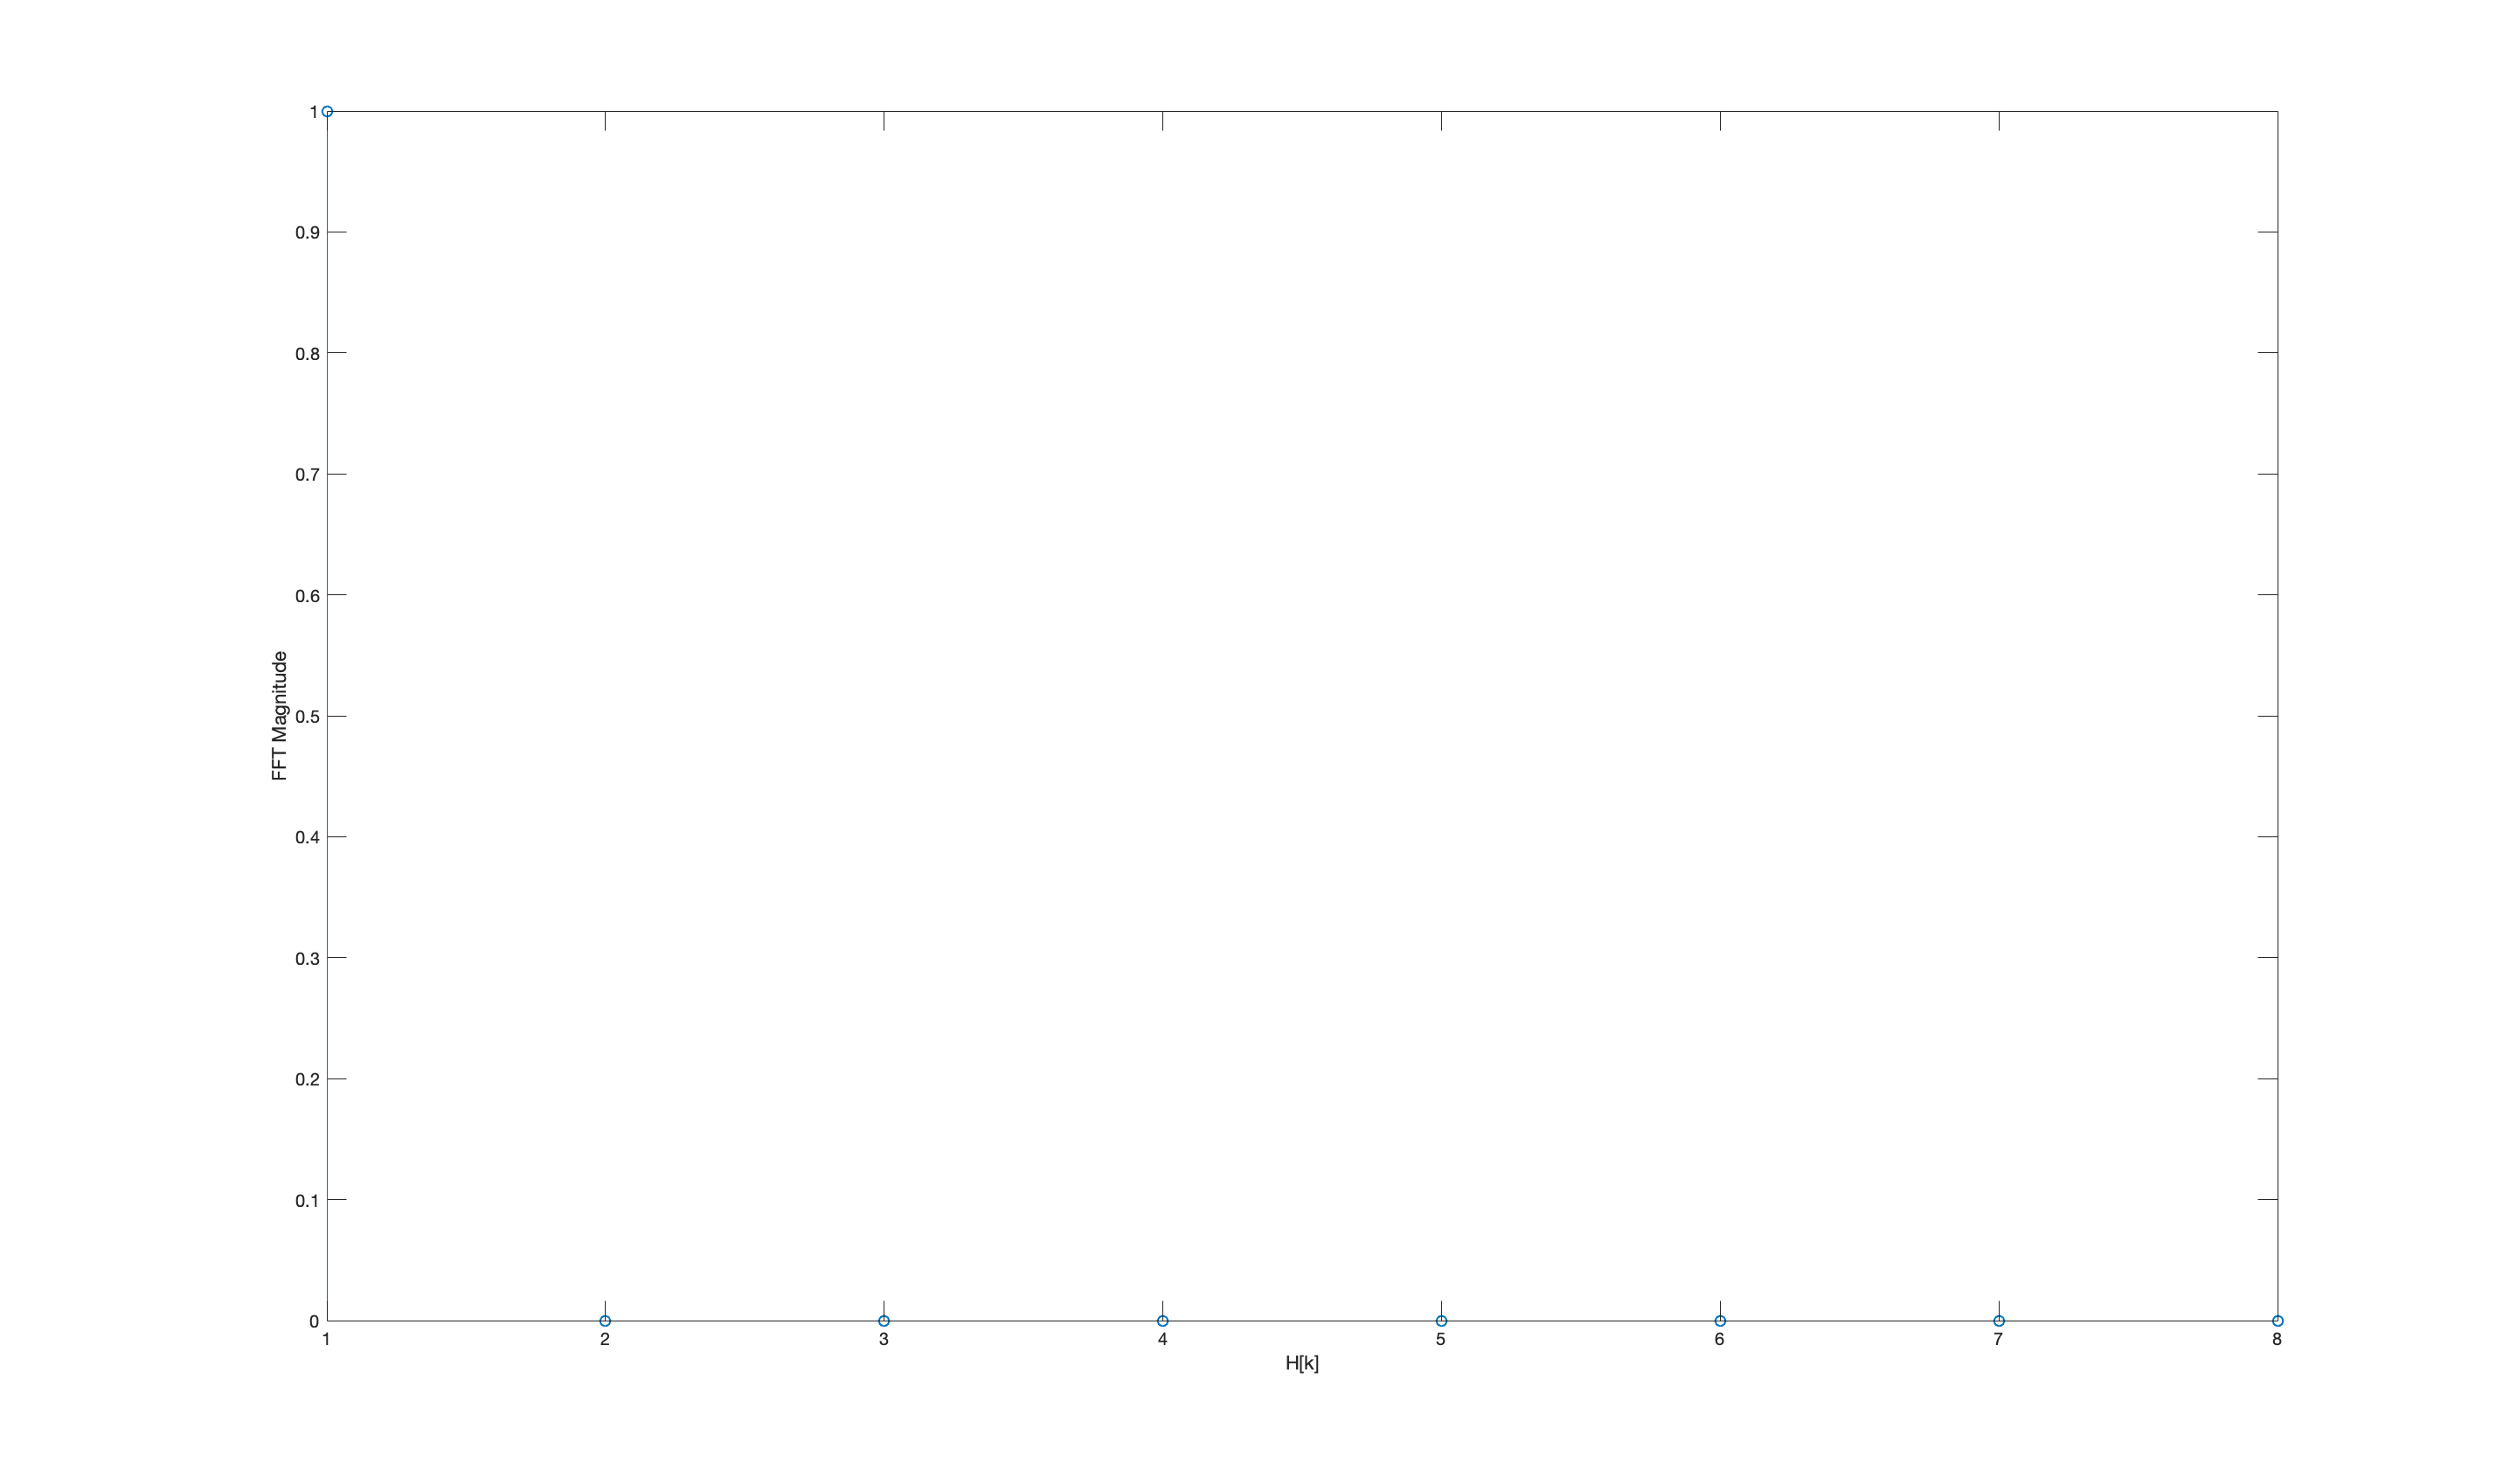
\includegraphics[width=1.0\textwidth]{./averaging_filter.png}
\caption{7.1) FFT of filter h}
\end{figure}

\begin{figure}[h!]
\centering
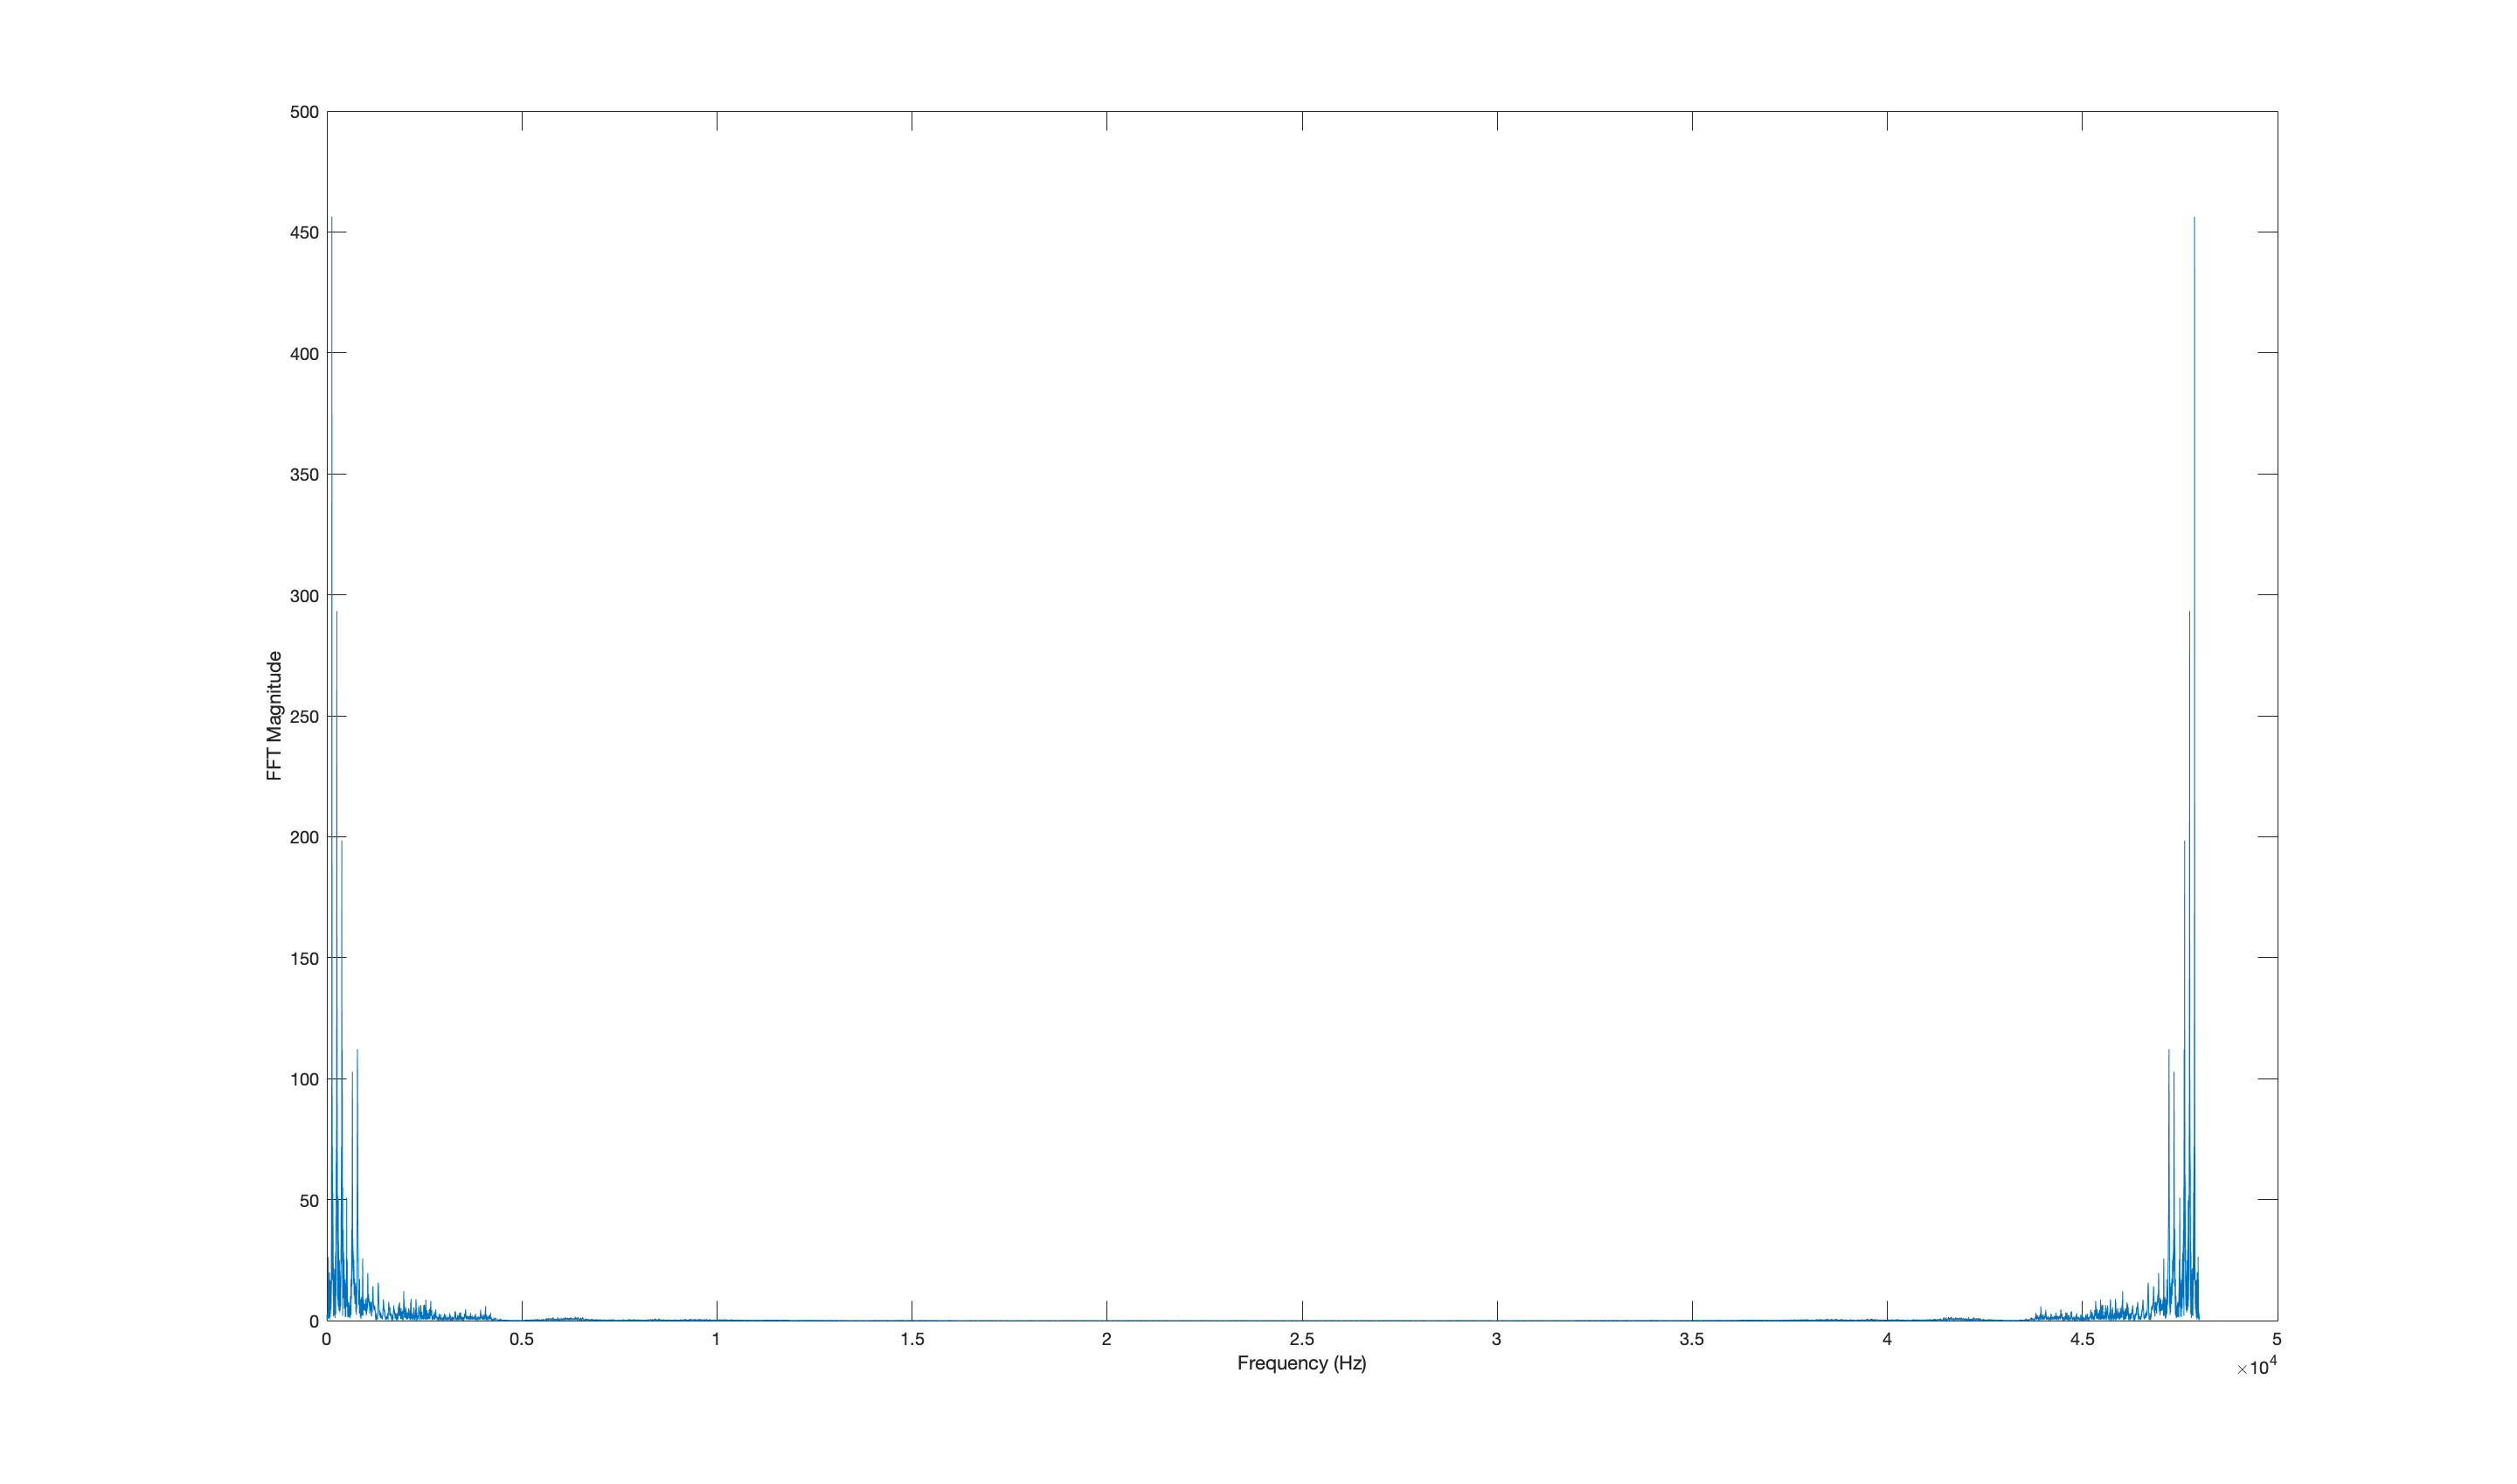
\includegraphics[width=1.0\textwidth]{./myvoice.png}
\caption{7.2) FFT of my voice}
\end{figure}

\begin{figure}[h!]
\centering
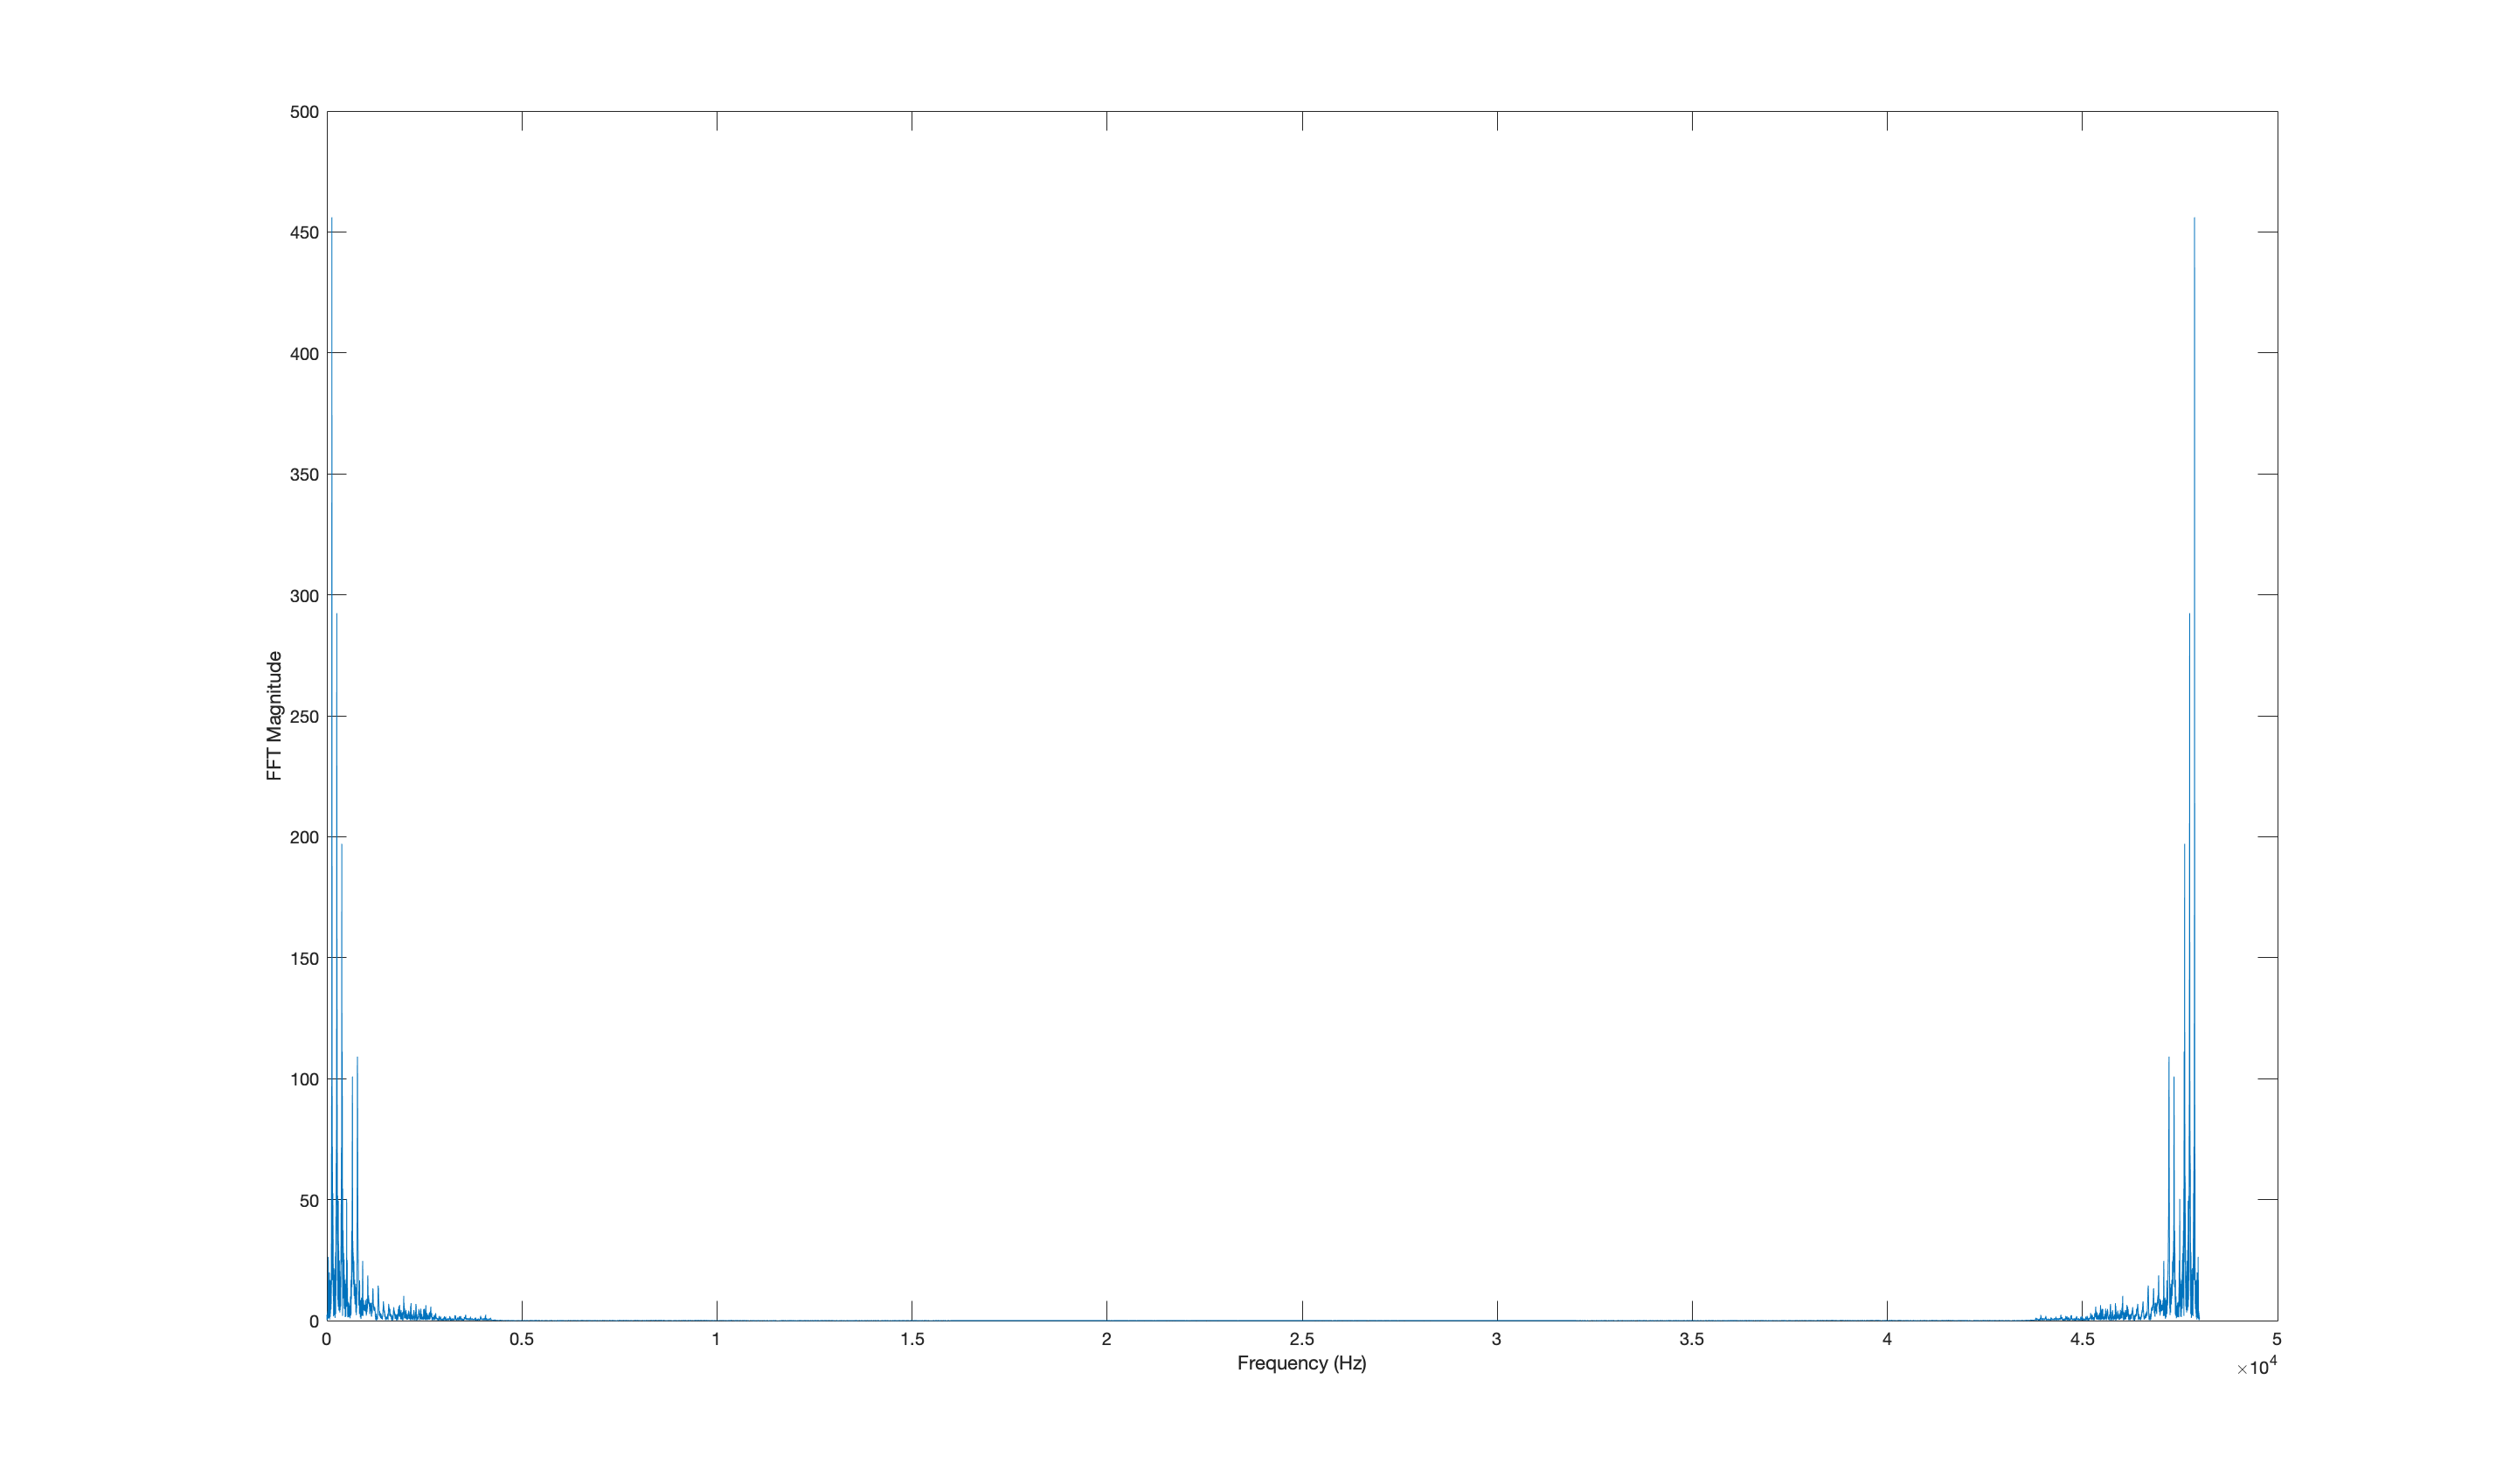
\includegraphics[width=1.0\textwidth]{./convolved_voice.png}
\caption{7.3) FFT of my voice convolved with filter h}
\end{figure}


------------

%%%%%%%%%%%%%%%%%%%%%%%%%%%%%%%%%%%%%%%%%%%%%%%%%%%%%%%%%%%%%%%%%%%%%%%%%%%%%%%%%%%%%%%%%%%%%%%%%%%%%%
 


\end{document}